\documentclass[11pt,a4paper]{article}
\usepackage[margin=2.3cm]{geometry}
\usepackage{amsmath,amssymb}
\usepackage{graphicx}
\usepackage{booktabs}
\usepackage{longtable}
\usepackage{array}
\usepackage{enumitem}
\usepackage{xcolor}
\usepackage{listings}
\usepackage{url}
\usepackage[hidelinks]{hyperref}
\usepackage{parskip}
\graphicspath{{../paper/figures/}{figures/}}
% Generated by scripts/make_figures.py from results/*.csv. Do not edit by hand.
\newcommand{\AddLastBaDij}{1.0}
\newcommand{\AddLastBaDijDK}{1.0}
\newcommand{\AddLastBaTwoFive}{2.2}
\newcommand{\AddLastBaTwoSix}{4.6}
\newcommand{\AddLastGridDij}{1.0}
\newcommand{\AddLastGridDijDK}{1.0}
\newcommand{\AddLastGridTwoFive}{4.3}
\newcommand{\AddLastGridTwoSix}{5.0}
\newcommand{\AddLastHubDij}{1.0}
\newcommand{\AddLastHubDijDK}{1.0}
\newcommand{\AddLastHubTwoFive}{3.3}
\newcommand{\AddLastHubTwoSix}{5.6}
\newcommand{\AddLastRandDij}{1.0}
\newcommand{\AddLastRandDijDK}{1.0}
\newcommand{\AddLastRandTwoFive}{3.1}
\newcommand{\AddLastRandTwoSix}{4.2}
\newcommand{\AddRatioMaxTwoFive}{4.4}
\newcommand{\AddRatioMaxTwoSix}{5.1}
\newcommand{\AddRatioMinTwoFive}{3.3}
\newcommand{\AddRatioMinTwoSix}{4.0}
\newcommand{\AllRatioMax}{8.7}
\newcommand{\AllRatioMin}{1.2}
\newcommand{\ChainNets}{CAL and NA}
\newcommand{\ChainPctA}{93.5}
\newcommand{\ChainPctB}{94.8}
\newcommand{\ChainRatioMax}{8.0}
\newcommand{\ChainRatioMin}{6.7}
\newcommand{\ChainRestMax}{53}
\newcommand{\ChainRestMin}{17}
\newcommand{\CmpLastBaDij}{14.2}
\newcommand{\CmpLastBaDijDK}{10.6}
\newcommand{\CmpLastBaTwoFive}{9.5}
\newcommand{\CmpLastBaTwoSix}{13.0}
\newcommand{\CmpLastGridDij}{9.0}
\newcommand{\CmpLastGridDijDK}{6.8}
\newcommand{\CmpLastGridTwoFive}{11.0}
\newcommand{\CmpLastGridTwoSix}{11.0}
\newcommand{\CmpLastHubDij}{16.2}
\newcommand{\CmpLastHubDijDK}{11.1}
\newcommand{\CmpLastHubTwoFive}{46.6}
\newcommand{\CmpLastHubTwoSix}{31.0}
\newcommand{\CmpLastRandDij}{17.1}
\newcommand{\CmpLastRandDijDK}{14.0}
\newcommand{\CmpLastRandTwoFive}{11.7}
\newcommand{\CmpLastRandTwoSix}{13.3}
\newcommand{\CmpRandTwentyDij}{15.5}
\newcommand{\CmpRandTwentyTwoFive}{9.7}
\newcommand{\CmpRandTwentyTwoSix}{14.9}
\newcommand{\CmpRangeBaTwoFiveMax}{12}
\newcommand{\CmpRangeBaTwoFiveMin}{10}
\newcommand{\CmpRangeBaTwoSixMax}{13}
\newcommand{\CmpRangeBaTwoSixMin}{11}
\newcommand{\CmpRangeRandTwoFiveMax}{12}
\newcommand{\CmpRangeRandTwoFiveMin}{10}
\newcommand{\CmpRangeRandTwoSixMax}{15}
\newcommand{\CmpRangeRandTwoSixMin}{12}
\newcommand{\CmpRatioMaxTwoFive}{2.66}
\newcommand{\CmpRatioMaxTwoSix}{2.15}
\newcommand{\CmpRatioMinTwoFive}{1.39}
\newcommand{\CmpRatioMinTwoSix}{1.63}
\newcommand{\CrossCmpBaTwoFiveDij}{16}
\newcommand{\CrossCmpBaTwoFiveDijDK}{20}
\newcommand{\CrossCmpBaTwoSixDij}{20}
\newcommand{\CrossCmpBaTwoSixDijDK}{none}
\newcommand{\CrossCmpGridTwoFiveDij}{none}
\newcommand{\CrossCmpGridTwoFiveDijDK}{none}
\newcommand{\CrossCmpGridTwoSixDij}{none}
\newcommand{\CrossCmpGridTwoSixDijDK}{none}
\newcommand{\CrossCmpHubTwoFiveDij}{none}
\newcommand{\CrossCmpHubTwoFiveDijDK}{none}
\newcommand{\CrossCmpHubTwoSixDij}{none}
\newcommand{\CrossCmpHubTwoSixDijDK}{none}
\newcommand{\CrossCmpRandTwoFiveDij}{14}
\newcommand{\CrossCmpRandTwoFiveDijDK}{17}
\newcommand{\CrossCmpRandTwoSixDij}{20}
\newcommand{\CrossCmpRandTwoSixDijDK}{22}
\newcommand{\CrossOpsBaTwoFiveDij}{18}
\newcommand{\CrossOpsBaTwoFiveDijDK}{none}
\newcommand{\CrossOpsBaTwoSixDij}{none}
\newcommand{\CrossOpsBaTwoSixDijDK}{none}
\newcommand{\CrossOpsGridTwoFiveDij}{none}
\newcommand{\CrossOpsGridTwoFiveDijDK}{none}
\newcommand{\CrossOpsGridTwoSixDij}{none}
\newcommand{\CrossOpsGridTwoSixDijDK}{none}
\newcommand{\CrossOpsHubTwoFiveDij}{none}
\newcommand{\CrossOpsHubTwoFiveDijDK}{none}
\newcommand{\CrossOpsHubTwoSixDij}{none}
\newcommand{\CrossOpsHubTwoSixDijDK}{none}
\newcommand{\CrossOpsRandTwoFiveDij}{16}
\newcommand{\CrossOpsRandTwoFiveDijDK}{18}
\newcommand{\CrossOpsRandTwoSixDij}{22}
\newcommand{\CrossOpsRandTwoSixDijDK}{none}
\newcommand{\DensHighTwoFive}{1.6}
\newcommand{\DensHighTwoSix}{2.3}
\newcommand{\DensLowTwoFive}{2.2}
\newcommand{\DensLowTwoSix}{3.6}
\newcommand{\DensMaxTwoFive}{2.2}
\newcommand{\DensMaxTwoSix}{3.6}
\newcommand{\DensMinTwoFive}{1.5}
\newcommand{\DensMinTwoSix}{2.3}
\newcommand{\DkLargeMax}{2.1}
\newcommand{\DupPctMaxTwoFive}{1.0}
\newcommand{\DupPctMaxTwoSix}{0.9}
\newcommand{\DupPctMinTwoFive}{0.1}
\newcommand{\DupPctMinTwoSix}{0.0}
\newcommand{\FaceValueCrossLog}{982}
\newcommand{\GainTwoFiveAtSixtyFour}{4.0}
\newcommand{\GainTwoFiveAtTwenty}{2.7}
\newcommand{\GainTwoSixAtSixtyFour}{3.3}
\newcommand{\GainTwoSixAtTwenty}{2.2}
\newcommand{\GridLateMax}{3.8}
\newcommand{\GridLateMin}{2.7}
\newcommand{\HubCmpDij}{14}
\newcommand{\HubCmpRatioMaxTwoFive}{2.9}
\newcommand{\HubCmpRatioMaxTwoSix}{2.2}
\newcommand{\HubCmpRatioMinTwoFive}{2.4}
\newcommand{\HubCmpRatioMinTwoSix}{1.9}
\newcommand{\HubCmpTwoFive}{38}
\newcommand{\HubCmpTwoSix}{26}
\newcommand{\HubRedCmpDij}{118}
\newcommand{\HubRedCmpTwoFive}{98}
\newcommand{\HubRedCmpTwoSix}{55}
\newcommand{\HubRedDijSlow}{6.7}
\newcommand{\HubRedSameTwoFive}{2.9}
\newcommand{\HubRedSameTwoSix}{2.5}
\newcommand{\MainScanMaxTwoFive}{2.8}
\newcommand{\MainScanMaxTwoSix}{4.0}
\newcommand{\MainScanMinTwoFive}{2.1}
\newcommand{\MainScanMinTwoSix}{3.0}
\newcommand{\MemDij}{501}
\newcommand{\MemRatioTwoFive}{1.7}
\newcommand{\MemRatioTwoSix}{2.3}
\newcommand{\MemTwoFive}{859}
\newcommand{\MemTwoSix}{1170}
\newcommand{\MsSixteenDij}{6}
\newcommand{\MsSixteenTwoFive}{11}
\newcommand{\MsTwentyDij}{271}
\newcommand{\MsTwentyTwoDij}{1866}
\newcommand{\MsTwentyTwoFive}{454}
\newcommand{\MsTwentyTwoTwoFive}{2805}
\newcommand{\OpsRandTwentyDij}{16.5}
\newcommand{\OpsRandTwentyTwoFive}{11.9}
\newcommand{\OpsRandTwentyTwoSix}{19.8}
\newcommand{\OpsRatioMaxTwoFive}{2.9}
\newcommand{\OpsRatioMaxTwoSix}{2.5}
\newcommand{\OpsRatioMinTwoFive}{1.6}
\newcommand{\OpsRatioMinTwoSix}{2.0}
\newcommand{\ParNATwoFiveBest}{3.94}
\newcommand{\ParNATwoFiveBestK}{6}
\newcommand{\ParNATwoFiveBestT}{5}
\newcommand{\ParNATwoFiveDefault}{6.44}
\newcommand{\ParNATwoFiveGain}{39}
\newcommand{\ParNATwoFiveWorst}{15.9}
\newcommand{\ParNATwoSixBest}{4.72}
\newcommand{\ParNATwoSixBestK}{4}
\newcommand{\ParNATwoSixBestT}{9}
\newcommand{\ParNATwoSixDefault}{6.80}
\newcommand{\ParNATwoSixGain}{31}
\newcommand{\ParNATwoSixWorst}{15.4}
\newcommand{\ParSFTwoFiveBest}{3.05}
\newcommand{\ParSFTwoFiveBestK}{5}
\newcommand{\ParSFTwoFiveBestT}{6}
\newcommand{\ParSFTwoFiveDefault}{3.46}
\newcommand{\ParSFTwoFiveGain}{12}
\newcommand{\ParSFTwoFiveWorst}{14.1}
\newcommand{\ParSFTwoSixBest}{4.09}
\newcommand{\ParSFTwoSixBestK}{3}
\newcommand{\ParSFTwoSixBestT}{9}
\newcommand{\ParSFTwoSixDefault}{4.62}
\newcommand{\ParSFTwoSixGain}{11}
\newcommand{\ParSFTwoSixWorst}{12.8}
\newcommand{\PeakBa}{51}
\newcommand{\PeakGrid}{0.1}
\newcommand{\PeakGridSmall}{7.5}
\newcommand{\PeakHub}{100}
\newcommand{\PeakRand}{33}
\newcommand{\PerOpMaxTwoFive}{2.9}
\newcommand{\PerOpMaxTwoSix}{2.7}
\newcommand{\PerOpMinTwoFive}{2.1}
\newcommand{\PerOpMinTwoSix}{2.3}
\newcommand{\PivotScanMaxTwoFive}{1.98}
\newcommand{\PivotScanMaxTwoSix}{0.72}
\newcommand{\PivotScanMinTwoFive}{1.16}
\newcommand{\PivotScanMinTwoSix}{0.02}
\newcommand{\PrintedTimeMaxTwoFive}{1.09}
\newcommand{\PrintedTimeMaxTwoSix}{1.01}
\newcommand{\PrintedTimeMinTwoFive}{0.98}
\newcommand{\PrintedTimeMinTwoSix}{0.97}
\newcommand{\RatioRandSixteenTwoFive}{1.9}
\newcommand{\RatioRandTwentyTwoFive}{1.7}
\newcommand{\RatioRandTwentyTwoTwoFive}{1.5}
\newcommand{\RealRatioMax}{8.0}
\newcommand{\RealRatioMaxTwoFive}{8.0}
\newcommand{\RealRatioMaxTwoSix}{6.7}
\newcommand{\RealRatioMin}{3.5}
\newcommand{\RealRatioMinTwoFive}{3.5}
\newcommand{\RealRatioMinTwoSix}{4.7}
\newcommand{\RealSources}{20}
\newcommand{\RealSrcMaxTwoFive}{9.5}
\newcommand{\RealSrcMaxTwoSix}{7.3}
\newcommand{\RealSrcMinTwoFive}{3.2}
\newcommand{\RealSrcMinTwoSix}{4.3}
\newcommand{\RealTwoSixFasterCount}{1}
\newcommand{\RealTwoSixFasterList}{CAL}
\newcommand{\RealTwoSixFasterWord}{one}
\newcommand{\RealTwoSixSlowerWord}{four}
\newcommand{\ReduceNGrowMax}{5.2}
\newcommand{\ReduceNGrowMin}{4.1}
\newcommand{\ReduceSlowMaxTwoFive}{5.6}
\newcommand{\ReduceSlowMaxTwoSix}{3.2}
\newcommand{\ReduceSlowMinTwoFive}{2.5}
\newcommand{\ReduceSlowMinTwoSix}{2.0}
\newcommand{\RestRatioMax}{5.1}
\newcommand{\RestRatioMin}{3.5}
\newcommand{\RoadPeakMax}{1.7}
\newcommand{\RoadPeakMin}{0.1}
\newcommand{\RoadsMoreAddsTwoSix}{four}
\newcommand{\RoadsMoreCmpTwoSix}{four}
\newcommand{\ScaleBaMaxExp}{21}
\newcommand{\ScaleBaTwoFiveArgmin}{21}
\newcommand{\ScaleBaTwoFiveFirst}{5.7}
\newcommand{\ScaleBaTwoFiveLast}{1.2}
\newcommand{\ScaleBaTwoFiveMax}{5.7}
\newcommand{\ScaleBaTwoFiveMin}{1.25}
\newcommand{\ScaleBaTwoSixArgmin}{21}
\newcommand{\ScaleBaTwoSixFirst}{6.3}
\newcommand{\ScaleBaTwoSixLast}{2.0}
\newcommand{\ScaleBaTwoSixMax}{6.3}
\newcommand{\ScaleBaTwoSixMin}{2.02}
\newcommand{\ScaleGridMaxExp}{22}
\newcommand{\ScaleGridTwoFiveArgmin}{18}
\newcommand{\ScaleGridTwoFiveFirst}{5.6}
\newcommand{\ScaleGridTwoFiveLast}{3.0}
\newcommand{\ScaleGridTwoFiveMax}{5.6}
\newcommand{\ScaleGridTwoFiveMin}{2.72}
\newcommand{\ScaleGridTwoSixArgmin}{18}
\newcommand{\ScaleGridTwoSixFirst}{6.0}
\newcommand{\ScaleGridTwoSixLast}{3.4}
\newcommand{\ScaleGridTwoSixMax}{6.0}
\newcommand{\ScaleGridTwoSixMin}{3.14}
\newcommand{\ScaleHubMaxExp}{21}
\newcommand{\ScaleHubTwoFiveArgmin}{21}
\newcommand{\ScaleHubTwoFiveFirst}{8.2}
\newcommand{\ScaleHubTwoFiveLast}{1.7}
\newcommand{\ScaleHubTwoFiveMax}{8.2}
\newcommand{\ScaleHubTwoFiveMin}{1.68}
\newcommand{\ScaleHubTwoSixArgmin}{21}
\newcommand{\ScaleHubTwoSixFirst}{8.7}
\newcommand{\ScaleHubTwoSixLast}{3.9}
\newcommand{\ScaleHubTwoSixMax}{8.7}
\newcommand{\ScaleHubTwoSixMin}{3.94}
\newcommand{\ScaleRandMaxExp}{22}
\newcommand{\ScaleRandTwoFiveArgmin}{22}
\newcommand{\ScaleRandTwoFiveFirst}{5.9}
\newcommand{\ScaleRandTwoFiveLast}{1.5}
\newcommand{\ScaleRandTwoFiveMax}{5.9}
\newcommand{\ScaleRandTwoFiveMin}{1.48}
\newcommand{\ScaleRandTwoSixArgmin}{22}
\newcommand{\ScaleRandTwoSixFirst}{6.8}
\newcommand{\ScaleRandTwoSixLast}{1.8}
\newcommand{\ScaleRandTwoSixMax}{6.8}
\newcommand{\ScaleRandTwoSixMin}{1.85}
\newcommand{\ScanLastBaDij}{1.0}
\newcommand{\ScanLastBaDijDK}{1.0}
\newcommand{\ScanLastBaTwoFive}{3.3}
\newcommand{\ScanLastBaTwoSix}{4.6}
\newcommand{\ScanLastGridDij}{1.0}
\newcommand{\ScanLastGridDijDK}{1.0}
\newcommand{\ScanLastGridTwoFive}{5.3}
\newcommand{\ScanLastGridTwoSix}{5.0}
\newcommand{\ScanLastHubDij}{1.0}
\newcommand{\ScanLastHubDijDK}{1.0}
\newcommand{\ScanLastHubTwoFive}{4.0}
\newcommand{\ScanLastHubTwoSix}{5.6}
\newcommand{\ScanLastRandDij}{1.0}
\newcommand{\ScanLastRandDijDK}{1.0}
\newcommand{\ScanLastRandTwoFive}{4.1}
\newcommand{\ScanLastRandTwoSix}{4.2}
\newcommand{\ScanMaxTwoFive}{4.8}
\newcommand{\ScanMaxTwoSix}{5.1}
\newcommand{\ScanMinTwoFive}{4.3}
\newcommand{\ScanMinTwoSix}{4.0}
\newcommand{\SlopeBaDij}{0.67}
\newcommand{\SlopeBaDijDK}{0.50}
\newcommand{\SlopeBaTwoFive}{-0.22}
\newcommand{\SlopeBaTwoSix}{0.09}
\newcommand{\SlopeGridDij}{0.33}
\newcommand{\SlopeGridDijDK}{0.26}
\newcommand{\SlopeGridTwoFive}{0.30}
\newcommand{\SlopeGridTwoSix}{0.16}
\newcommand{\SlopeHubDij}{0.75}
\newcommand{\SlopeHubDijDK}{0.50}
\newcommand{\SlopeHubTwoFive}{2.65}
\newcommand{\SlopeHubTwoSix}{0.96}
\newcommand{\SlopeRandDij}{0.80}
\newcommand{\SlopeRandDijDK}{0.67}
\newcommand{\SlopeRandTwoFive}{0.14}
\newcommand{\SlopeRandTwoSix}{-0.07}
\newcommand{\SnapBestInstance}{Pokec with random weights}
\newcommand{\SnapCmpOtherMaxTwoFive}{1.65}
\newcommand{\SnapCmpOtherMaxTwoSix}{2.91}
\newcommand{\SnapCmpOtherMinTwoFive}{0.79}
\newcommand{\SnapCmpOtherMinTwoSix}{1.23}
\newcommand{\SnapCmpRoadMaxTwoFive}{1.43}
\newcommand{\SnapCmpRoadMaxTwoSix}{1.61}
\newcommand{\SnapCmpRoadMinTwoFive}{1.09}
\newcommand{\SnapCmpRoadMinTwoSix}{1.22}
\newcommand{\SnapFewerCmpDKTwoFive}{none}
\newcommand{\SnapFewerCmpDKTwoSix}{none}
\newcommand{\SnapFewerCmpTwoFive}{two}
\newcommand{\SnapFewerCmpTwoSix}{none}
\newcommand{\SnapFewerListTwoFive}{Google and Pokec}
\newcommand{\SnapGraphs}{six}
\newcommand{\SnapInstances}{twelve}
\newcommand{\SnapOtherPeakMax}{50}
\newcommand{\SnapOtherPeakMin}{13}
\newcommand{\SnapRandCmpMaxTwoFive}{1.20}
\newcommand{\SnapRandCmpMaxTwoSix}{1.52}
\newcommand{\SnapRandCmpMinTwoFive}{0.79}
\newcommand{\SnapRandCmpMinTwoSix}{1.22}
\newcommand{\SnapRandTimeMaxTwoFive}{3.1}
\newcommand{\SnapRandTimeMaxTwoSix}{4.3}
\newcommand{\SnapRandTimeMinTwoFive}{1.3}
\newcommand{\SnapRandTimeMinTwoSix}{1.9}
\newcommand{\SnapRatioMaxTwoFive}{3.2}
\newcommand{\SnapRatioMaxTwoSix}{4.5}
\newcommand{\SnapRatioMinTwoFive}{1.3}
\newcommand{\SnapRatioMinTwoSix}{1.9}
\newcommand{\SnapRoadPeakMax}{0.3}
\newcommand{\SnapTimeOtherMaxTwoFive}{3.2}
\newcommand{\SnapTimeOtherMaxTwoSix}{4.5}
\newcommand{\SnapTimeOtherMinTwoFive}{1.3}
\newcommand{\SnapTimeOtherMinTwoSix}{1.9}
\newcommand{\SnapTimeRoadMaxTwoFive}{3.0}
\newcommand{\SnapTimeRoadMaxTwoSix}{3.8}
\newcommand{\SnapTimeRoadMinTwoFive}{2.6}
\newcommand{\SnapTimeRoadMinTwoSix}{3.3}
\newcommand{\SnapTwoSixFaster}{none}
\newcommand{\SnapUnitCmpMaxTwoFive}{1.65}
\newcommand{\SnapUnitCmpMaxTwoSix}{2.91}
\newcommand{\SnapUnitCmpMinTwoFive}{1.03}
\newcommand{\SnapUnitCmpMinTwoSix}{1.56}
\newcommand{\SnapUnitTimeMaxTwoFive}{3.2}
\newcommand{\SnapUnitTimeMaxTwoSix}{4.5}
\newcommand{\SnapUnitTimeMinTwoFive}{2.2}
\newcommand{\SnapUnitTimeMinTwoSix}{3.0}
\newcommand{\SynthPoints}{44}
\newcommand{\SynthTwoSixFasterCount}{0}
\newcommand{\TimeRandTwentyTwoFive}{1.7}
\newcommand{\TimeRandTwentyTwoSix}{2.7}
\newcommand{\ValMediumBoundTwoSix}{1\,435}
\newcommand{\ValMediumDupTwoFive}{9\,343}
\newcommand{\ValMediumDupTwoSix}{10\,510}
\newcommand{\ValMediumRuns}{510\,000}
\newcommand{\ValMediumStaleTwoFive}{10\,402}
\newcommand{\ValMediumStaleTwoSix}{10\,510}
\newcommand{\ValMediumTrials}{30\,000}
\newcommand{\ValMediumWrong}{0}
\newcommand{\ValMinNBoundTwoSix}{10}
\newcommand{\ValMinNDupTwoFive}{9}
\newcommand{\ValMinNDupTwoSix}{12}
\newcommand{\ValSmallBoundTwoSix}{8\,939}
\newcommand{\ValSmallDupTwoFive}{4\,788}
\newcommand{\ValSmallDupTwoSix}{3\,475}
\newcommand{\ValSmallRuns}{3\,400\,000}
\newcommand{\ValSmallStaleTwoFive}{5\,293}
\newcommand{\ValSmallStaleTwoSix}{3\,475}
\newcommand{\ValSmallTrials}{200\,000}
\newcommand{\ValSmallWrong}{0}
\newcommand{\WeightMaxTwoFive}{2.3}
\newcommand{\WeightMaxTwoSix}{3.8}
\newcommand{\WeightMinTwoFive}{1.9}
\newcommand{\WeightMinTwoSix}{2.8}
\newcommand{\WeightUnitTwoFive}{1.9}
\newcommand{\WeightUnitTwoSix}{2.8}
\newcommand{\WeightWideTwoFive}{1.9}
\newcommand{\WeightWideTwoSix}{3.0}

\lstset{basicstyle=\ttfamily\small,columns=fullflexible,breaklines=true,frame=single,framesep=4pt,
        xleftmargin=4pt,xrightmargin=4pt,backgroundcolor=\color{black!3},rulecolor=\color{black!25}}
\newcommand{\dhat}{\widehat{d}}
\newcommand{\code}[1]{\texttt{#1}}
\newcommand{\bmA}{BMSSP-25}
\newcommand{\bmB}{BMSSP-26}
\setlist{itemsep=2pt,topsep=4pt}
\sloppy\emergencystretch=4em

\title{Explanation\\[4pt]\large How the comparison of Dijkstra's algorithm with the two\\ Duan et al.\ shortest-path algorithms works}
\author{Companion guide to the research paper}
\date{12 October 2026\\[6pt]\normalsize Written for the author's own understanding; the paper does not refer to this document.}

\begin{document}
\maketitle
\tableofcontents
\newpage

\section{The project in one page}
\textbf{Question.} Dijkstra's algorithm (1959) has been the standard way to compute shortest paths from one source. In 2025 Duan, Mao, Mao, Shu and Yin published an algorithm that is \emph{asymptotically} faster on sparse graphs, $O(m\log^{2/3}n)$ instead of $O(m+n\log n)$, and in 2026 four of them improved it to $O(m\sqrt{\log n}+\sqrt{mn\log n\log\log n})$. Both papers are pure theory. The research paper asks: what do these two algorithms look like next to Dijkstra's algorithm in theory, and how do they behave when all three are actually implemented and run on the same graphs?

\textbf{What was done.}
\begin{enumerate}
\item Both new algorithms were implemented in C++ directly from the pseudocode in the two papers (files \code{scripts/src/bmssp25.hpp} and \code{scripts/src/bmssp26.hpp}), next to two versions of Dijkstra's algorithm (\code{dijkstra.hpp}).
\item The implementations were tested against an independent Bellman--Ford computation on \ValSmallTrials{} tiny and \ValMediumTrials{} medium random graphs, and against Dijkstra on every benchmark run. No run ever produced a wrong distance.
\item All algorithms were run on the five real road networks you specified (the SSTD~2005 collection from the \code{mehdi-ansari} repository) and on four families of generated graphs with up to $2^{22}\approx 4.2$ million vertices.
\item Two kinds of cost were measured: wall-clock time, and \emph{operation counts} (how many comparisons, additions and edge scans each algorithm performs). Counts do not depend on the computer, so they tell us whether a slowdown comes from the algorithm doing more work or from each step being more expensive.
\end{enumerate}

\textbf{Answer.} On every graph tested, Dijkstra's algorithm with an ordinary binary heap was the fastest (between \AllRatioMin{} and \AllRatioMax{} times faster). On the road networks it was \RealRatioMin{} to \RealRatioMax{} times faster, and there the new algorithms even perform more comparisons and 3--5 times more additions per edge, so they lose in the abstract cost model too. On large random graphs the picture in the abstract model is different: from a few tens of thousands of vertices on, the 2025 algorithm needs \emph{fewer} comparisons than Dijkstra, exactly as the theory predicts, but it is still slower on the clock (\ScaleRandTwoFiveLast{} times at four million vertices) because it looks at every edge 3--5 times and each of its steps is more expensive. The 2026 algorithm really does make the ``pivot finding'' step cheaper, as its authors intended, but it spends the saving elsewhere and was not faster than the 2025 algorithm in practice. While testing, two small inconsistencies in the 2026 pseudocode were found (Section~\ref{sec:fixes}); they do not make its answers wrong.

\textbf{Files.}
\begin{center}
\begin{tabular}{@{}p{5.2cm}p{9.8cm}@{}}
\toprule
\code{research-paper.pdf} & the paper (IEEE conference format, as in \code{Resources/format.docx})\\
\code{explanation.pdf} & this document\\
\code{figure\_data.txt} & every number plotted in the paper's figures, as plain text (Section~\ref{sec:figdata})\\
\code{paper/main.tex}, \code{paper/results\_rest.tex} & LaTeX source of the paper\\
\code{explanation/} & LaTeX source of this guide\\
\code{scripts/} & all code (Section~\ref{sec:code}) and the commands to reproduce (Section~\ref{sec:repro})\\
\code{results/} & every raw measurement as CSV, plus \code{summary.json}\\
\code{data/sstd2005/} & the downloaded road networks\\
\bottomrule
\end{tabular}
\end{center}

\section{Background: the problem and Dijkstra's algorithm}
\subsection{Shortest paths, labels and relaxation}
We are given a directed graph with $n$ vertices and $m$ edges (the paper says ``arcs''); every edge $(u,v)$ has a weight $w_{uv}\ge 0$. We want the length $d(v)$ of the shortest path from a source $s$ to every vertex $v$.

Every algorithm in this project keeps, for each vertex, a \emph{label} $\dhat[v]$: the length of the best path to $v$ found so far. Initially $\dhat[s]=0$ and all other labels are $\infty$. The only way a label changes is by \emph{relaxing} an edge $(u,v)$: if $\dhat[u]+w_{uv}$ is smaller than $\dhat[v]$, set $\dhat[v]$ to it. Labels therefore only go down and are never below the true distance. A vertex is called \emph{complete} once $\dhat[v]=d(v)$.

\subsection{Dijkstra's algorithm and the ``sorting barrier''}
Dijkstra's algorithm keeps all labelled but unfinished vertices in a priority queue. It repeatedly takes out the vertex with the smallest label (that vertex is guaranteed to be complete) and relaxes its outgoing edges. Every edge is looked at exactly once.

The catch is the priority queue. Vertices come out in increasing order of distance, so the algorithm sorts the vertices as a side effect, and sorting $n$ numbers by comparisons needs about $n\log n$ comparisons. This is the ``sorting barrier''. With a Fibonacci heap the total time is $O(m+n\log n)$; with a simple binary heap it is $O((m+n)\log n)$, which is what everybody uses in practice because binary heaps are fast.

In 2024 Haeupler et al.\ proved that Dijkstra's algorithm is optimal \emph{if the output has to list the vertices in order of distance}. The new algorithms escape this by returning only the distances, never the order.

\subsection{The comparison-addition model}
The bounds above are stated in a model where the only things one may do with weights are add two of them and compare two of them, each at unit cost. This is why the project counts comparisons and additions: they are the ``currency'' of the theorems.

\section{How the two new algorithms work}
\textbf{A note on names.} Neither Duan et al.\ paper gives its algorithm a name; they only name the recursive procedure inside both, BMSSP. Other authors therefore call the 2025 algorithm simply ``BMSSP''. Because this project compares two of them, the paper defines its own labels once, in the Introduction: \bmA{} is the algorithm of Duan, Mao, Mao, Shu and Yin (STOC 2025) and \bmB{} is the algorithm of Duan, Mao, Shu and Yin (ICALP 2026). The paper uses only these two names; this guide also says ``the 2025 algorithm'' and ``the 2026 algorithm'' where that reads more easily.

\subsection{The shared idea: solve bounded sub-problems recursively}
Call the set of labelled-but-unfinished vertices the \emph{frontier}. Dijkstra needs the minimum of the frontier at every step, which forces it to keep the whole frontier ordered. The new algorithms avoid this with two ideas.

\textbf{Idea 1: bounded multi-source shortest path (BMSSP).} Instead of asking for one vertex at a time, ask a bigger question: \emph{given a set $S$ of frontier vertices and a bound $B$, complete every vertex whose true distance is below $B$ and whose shortest path passes through $S$.} This question is answered recursively. A call
\[
\textsc{BMSSP}(\text{level } l,\ \text{bound } B,\ \text{frontier } S)
\]
repeatedly (a) takes the roughly $M$ smallest vertices $S_i$ out of its frontier, together with a value $B_i$ that separates them from the rest; (b) calls $\textsc{BMSSP}(l-1,B_i,S_i)$, which returns a set $U_i$ of now-complete vertices; (c) relaxes all edges leaving $U_i$ and puts the improved neighbours into its frontier. Level $0$ is a small Dijkstra search. The whole problem is one call with $S=\{s\}$ and $B=\infty$.

The data structure holding the frontier only has to deliver ``the $M$ smallest, in any order'', not a sorted sequence. It stores keys in \emph{blocks}; blocks are ordered among each other but unsorted inside. That is cheaper than a heap.

A call may also stop early when it has completed ``enough'' vertices (a \emph{partial execution}); it then returns a smaller bound $B'<B$ meaning ``everything below $B'$ is finished''.

\textbf{Idea 2: shrink the frontier to pivots.} If every frontier vertex went through the recursion, the recursion would in the end sort them and nothing would be gained. So each call first reduces its frontier $S$ to a much smaller set, by a factor of about $k$. The two algorithms differ mainly in how they do this.

\subsection{The 2025 algorithm (\bmA)}
\textbf{FindPivots.} Starting from $S$, relax edges outward for $k$ rounds (like $k$ rounds of the Bellman--Ford algorithm), only following labels below $B$. Let $W$ be all vertices touched.
\begin{itemize}
\item If $W$ grew larger than $k\cdot|S|$, the frontier is already small compared with the work to be done; keep all of $S$ as pivots.
\item Otherwise look at the edges that are currently ``tight'' ($\dhat[v]=\dhat[u]+w_{uv}$) inside $W$. They form a forest. A vertex of $S$ becomes a \emph{pivot} only if it is the root of a tree with at least $k$ vertices. Why is this safe? If the shortest path of some vertex leaves $S$ through a root whose tree has fewer than $k$ vertices, that path has fewer than $k$ edges inside the region and the $k$ rounds have already made the vertex complete.
\end{itemize}
Since every pivot ``owns'' at least $k$ vertices of $W$, there are at most $|W|/k$ pivots.

\textbf{The data structure $D$} (Lemma~3.3 of the paper) supports \textsc{Insert} (a single key), \textsc{BatchPrepend} (many keys that are all smaller than everything stored) and \textsc{Pull} (remove and return the $M$ smallest keys and a separating value). Internally it is two lists of blocks: one for batch-prepended keys and one for inserted keys, the latter indexed by a balanced search tree over block upper bounds. Blocks that overflow are split at their median, found by a linear-time selection algorithm.

\textbf{The main loop.} Insert the pivots into $D$. While $D$ is not empty and fewer than $k2^{lt}$ vertices have been completed: \textsc{Pull} $S_i,B_i$; recurse; relax the edges out of $U_i$. An improved neighbour whose new label is at least $B_i$ is inserted; one whose label lies between the returned $B_i'$ and $B_i$ is collected and batch-prepended, together with the vertices of $S_i$ that the sub-call did not finish.

\textbf{Base case.} A Dijkstra search from the single vertex in $S$ that stops after $k+1$ vertices.

\textbf{Parameters.} $k=\lfloor\log^{1/3}n\rfloor$, $t=\lfloor\log^{2/3}n\rfloor$, number of levels $\lceil\log n/t\rceil$, block size $M=2^{(l-1)t}$ at level $l$. For a million vertices this means $k=2$, $t=7$ and three levels.

\subsection{The 2026 algorithm (\bmB): what changes}
\textbf{Cheaper pivot finding.} The $k$ Bellman--Ford rounds cost about $k$ units of work per vertex. The 2026 paper observes that they compute more than needed. Its FindPivots instead runs, from each vertex $x$ of $S$, a tiny Dijkstra search that stops as soon as it has discovered $k$ vertices. Three things can happen:
\begin{itemize}
\item the search finds $k$ vertices: the little tree it explored is kept;
\item the search runs into a tree kept earlier: the two are glued together and the search stops;
\item the search runs out of vertices before reaching $k$: then everything reachable from $x$ below $B$ has just been finished; $x$ is put aside in a set $Q$ and its vertices in $W$.
\end{itemize}
The kept trees form a forest that connects the frontier. It is then cut into pieces of between $k$ and $3k$ vertices (Algorithm~5 of the paper, a depth-first traversal). The frontier vertices in one piece form a group $P_j$, and only the smallest member $p_j$ of each group is stored in $D$. When $p_j$ is pulled, the algorithm scans its group and takes along all members below the separator. So $D$ again holds only about a $1/k$ fraction of the frontier, but finding the groups cost only about $\log k$ per vertex.

\textbf{Simpler data structure.} One search tree of blocks. Operations: \textsc{Insert}, \textsc{Pull}, and \textsc{Merge}, which absorbs a whole smaller structure whose keys are all below the stored ones. A recursive call now \emph{returns its leftover frontier} as such a structure and the caller merges it; this replaces the \textsc{BatchPrepend} bookkeeping of 2025.

\textbf{Different sizes.} Block size $M=t\,2^{(l-1)t}$; a call stops after completing more than $t^3 2^{lt}$ vertices; the base case is a Dijkstra search (on a search tree) that completes up to $t^3+1$ vertices and may start from several vertices. Parameters: $t=\lceil\sqrt{\log n\log\log n/\delta}\,\rceil$ and $k=\lceil t/\log t\rceil$, where $\delta$ is the degree bound discussed next. For a million vertices: $t=6$, $k=3$, four levels, base case of up to 217 vertices.

\subsection{Two assumptions both papers make}
\textbf{All path lengths are different.} The proofs need that no two paths have the same length (otherwise ``the shortest-path tree'' is not unique). Real graphs have ties. Both papers therefore compare \emph{tuples} instead of numbers: (length, number of edges on the path, the vertex itself, its predecessor), lexicographically. In the code this is the type \code{Label} in \code{common.hpp}. It makes every label four fields wide and every comparison slower than Dijkstra's comparison of two plain numbers.

\textbf{Small degrees.} The running-time proofs assume that every vertex has only a few edges. A graph can be forced into this shape by replacing each vertex by a ring of zero-weight edges, one ring vertex per incident edge. For $\delta=3$ this roughly doubles-to-quintuples the number of vertices (it becomes $2m$) and triples the number of edges. The code can do this (\code{reduceDegree} in \code{graphs.hpp}, option \code{--reduce}); the main experiments do not, because it makes everything much slower (Table~VII of the paper).

\section{A worked mini-example of pivot finding}
Take $k=2$, bound $B=\infty$, and suppose the source's edges have been relaxed so that the frontier is $S=\{a,b\}$ with $\dhat[a]=1$, $\dhat[b]=4$. Edges: $a\to c$ (weight 2), $c\to d$ (1), $d\to e$ (3); $b$ has no outgoing edges.

\emph{2025 FindPivots.} Round 1 relaxes the edges out of $a$ and $b$: $c$ gets label $3$. Now $W=\{a,b,c\}$. Round 2 relaxes the edges out of $c$: $d$ gets label $4$. $W=\{a,b,c,d\}$, which is not larger than $k|S|=4$, so the forest rule applies. Tight edges: $a\to c$, $c\to d$. Trees: $\{a,c,d\}$ rooted at $a$ (3 vertices) and $\{b\}$ (1 vertex). Only $a$ has a tree with at least $k=2$ vertices, so the pivot set is $P=\{a\}$. Vertex $b$ is dropped from the frontier: it is complete and nothing below $B$ hangs under it. Note that the two rounds cost one relaxation attempt per edge out of $a,b,c$.

\emph{2026 FindPivots.} Search from $a$: discover $c$ (now 2 vertices $=k$), stop; tree $\{a,c\}$ is kept. Search from $b$: nothing reachable, fewer than $k$ vertices, so $b$ goes to $Q$ and $W=\{b\}$. The forest $\{a,c\}$ is one piece; its only frontier vertex is $a$, so the single group is $P_1=\{a\}$ with representative $a$. Same outcome, but edge $c\to d$ was not touched.

\section{The code}\label{sec:code}
Everything is in \code{scripts/}. The C++ part is header-only plus one driver.

\begin{longtable}{@{}p{3.6cm}p{11.6cm}@{}}
\toprule
File & What it contains\\
\midrule
\code{src/common.hpp} & Graph in compressed-sparse-row form (\code{Graph}); the tie-breaking label (\code{Label}, \code{lt}); per-vertex label storage (\code{LabelArray}); the operation counters (\code{Counters}, macro \code{CNT}); the worst-case linear selection routine \code{select\_kth}; a small random generator.\\
\code{src/dijkstra.hpp} & \code{DijkstraLazy}: binary heap of (key, vertex) pairs; outdated entries are skipped when popped. \code{DijkstraIndexed}: heap with positions, supports DecreaseKey.\\
\code{src/bmssp25.hpp} & \code{BlockSeq25}: the Lemma~3.3 structure (\code{insert}, \code{batchPrepend}, \code{pull}, \code{erase}). \code{Bmssp25}: \code{findPivots} (Algorithm~1), \code{baseCase} (Algorithm~2), \code{bmssp} (Algorithm~3), \code{run}.\\
\code{src/bmssp26.hpp} & \code{BlockTree26}: the Lemma~3.4 structure (\code{insert}, \code{merge}, \code{pull}, \code{erase}, \code{exportTo}). \code{BaseSet26}: search tree for the base case. \code{Bmssp26}: \code{findPivots} (Algorithm~2 followed by the partition of Algorithm~5), \code{selectPivot}, \code{baseCase} (Algorithm~4), \code{bmssp} (Algorithm~3), \code{run}.\\
\code{src/graphs.hpp} & Loader for the road-network files (\code{loadSSTD}); generators \code{genRandom}, \code{genGrid}, \code{genBA}, \code{genHub}; the degree reduction \code{reduceDegree}.\\
\code{src/main.cpp} & Command-line driver with three commands: \code{info}, \code{run}, \code{validate}.\\
\code{Makefile} & Builds \code{bin/sssp} (timing), \code{bin/sssp\_count} (same code with counters, \code{-DCOUNT\_OPS}) and \code{bin/sssp\_debug} (address and undefined-behaviour sanitizers).\\
\code{fetch\_data.sh} & Clones the data repository at the exact commit used.\\
\code{run\_experiments.py} & Runs every experiment and writes \code{results/*.csv}.\\
\code{make\_figures.py} & Reads the CSV files and writes the figures, the table bodies and \code{paper/numbers.tex}.\\
\code{build\_pdfs.sh} & Runs \code{make\_figures.py} and typesets the paper and this guide.\\
\bottomrule
\end{longtable}

\subsection{Design decisions worth knowing}
\begin{itemize}
\item \textbf{Exact arithmetic.} Road lengths in the data have six decimals; they are multiplied by $10^6$ and stored as 64-bit integers. Sums are exact, so two algorithms either agree exactly or one is wrong.
\item \textbf{One label array.} \code{LabelArray::d[v]} holds (length, hops, predecessor). \code{through(u,v,w)} builds the candidate label of $v$ via $u$ and counts one addition; \code{notWorse(c)} checks ``candidate $\le$ current label'' and counts one comparison.
\item \textbf{Sets $U$ without copying.} Every call appends the vertices it completes to one global array \code{Ubuf} and returns only the index range. A parent's set is automatically the concatenation of its children's ranges.
\item \textbf{Finding a key in $O(1)$.} For each recursion level there is an array that says in which block and at which position a vertex is stored (a direct-address table). This works because calls on the same level never overlap in time.
\item \textbf{Stamps instead of clearing.} ``Is $v$ in set $X$?'' is answered by comparing \code{stamp[v]} with a counter that is increased whenever a new set starts, so sets never have to be erased.
\item \textbf{Selection.} \code{select\_kth} is quickselect; if it has done more than a linear amount of work it switches to the median-of-medians rule, which guarantees linear time in the worst case, as the proofs require.
\end{itemize}

\subsection{From pseudocode line to code}
\begin{longtable}{@{}p{6.4cm}p{8.8cm}@{}}
\toprule
Paper & Code\\
\midrule
2025, Alg.~1 lines 4--14 ($k$ relaxation rounds) & \code{Bmssp25::findPivots}, loop \code{for (int i = 1; i <= k; i++)}\\
2025, Alg.~1 lines 15--16 (forest, pivots) & same function, after the loop: \code{par}, \code{rootOf}, \code{tsize}\\
2025, Alg.~2 (base case) & \code{Bmssp25::baseCase}\\
2025, Alg.~3 lines 8--21 (main loop) & \code{Bmssp25::bmssp}, the \code{while} loop\\
2025, Lemma~3.3 & class \code{BlockSeq25}\\
2026, Alg.~1 (Relax) & \code{Bmssp26::relax}\\
2026, Alg.~2 lines 2--18 (local searches) & \code{Bmssp26::findPivots}, loop over \code{S}\\
2026, Alg.~2 line 20 and Alg.~5 (partition) & same function, part ``partition the forest''\\
2026, Alg.~2 lines 21--22 (groups $P_j$) & same function, last loop\\
2026, Alg.~3 lines 9--30 (main loop) & \code{Bmssp26::bmssp}, the \code{while} loop\\
2026, Alg.~3 lines 31--38 (finalization) & same function, after the loop\\
2026, Alg.~4 (base case) & \code{Bmssp26::baseCase}\\
2026, Lemma~3.4 and Appendix~A.2 & classes \code{BlockTree26} and \code{BaseSet26}\\
\bottomrule
\end{longtable}
(Line and lemma numbers are those of the arXiv versions 2504.17033v2 and 2602.07868v2. The published ICALP version of the 2026 paper uses the same line numbers but numbers its lemmas consecutively: Lemma~3.1 there is Lemma~3, Lemma~3.4 is Lemma~6, Lemma~3.7 is Lemma~9 and Lemma~3.8 is Lemma~10. The research paper cites the published numbering.)

\section{Three places where the code deliberately differs from the printed pseudocode}\label{sec:fixes}
Each difference can be switched off on the command line (\code{--nofix}, \code{--literal-base}), and the validation counts how often it matters.

\subsection{Deleting completed vertices from $D$ (both algorithms)}
A key in $D$ keeps the value it had when it was inserted. During a recursive call the label of that vertex can drop, and the vertex can even be completed by the call, while its old entry is still in the caller's $D$. Later the old entry is pulled and the vertex's already finished subtree is explored again.

For the 2025 algorithm this was found by Castro, Clementino and de Freitas (arXiv:2511.03007); they report that the original authors confirmed the problem and the fix, which is to delete a vertex from $D$ as soon as it is reported complete. The code does that in \code{Bmssp25::bmssp} (\code{if (fix) D.erase(u)}).

The 2026 paper says in the proof of its correctness lemma ``$U_i$ is not in $D$, no need to remove''. The instrumented runs show otherwise: in \ValSmallStaleTwoSix{} of the \ValSmallTrials{} tiny graphs and \ValMediumStaleTwoSix{} of the \ValMediumTrials{} medium graphs a vertex of $U_i$ was still stored in the caller's $D$ when the sub-call returned (counter \code{stale\_parent}, measured before anything is merged, so it is not an artefact of the merge). Without deletion, vertices get reported complete twice (\code{dup\_u}). The smallest example found has \ValMinNDupTwoSix{} vertices and is saved in \code{results/validation/witness\_2026\_duplicate\_U.txt}. The code applies the same deletion as for 2025.

\emph{How sure is this?} The observation is a measurement on my implementation of the pseudocode; I re-read the pseudocode against the code line by line, and the mechanism (keys are not updated when labels drop) is plain from the pseudocode. But the authors have not been asked, so the paper words it as an observation, not as a confirmed erratum. The distances were correct in every run either way.

\subsection{The boundary returned by the 2026 base case}
Algorithm~4 does, in a loop: pull the smallest vertex $u$ \emph{and a separator $B'$}; add $u$ to $U$; relax the edges of $u$ (which inserts new keys). It then returns the last $B'$. But that $B'$ was computed before the edges of the last vertex were relaxed. If the loop ends because the size limit $t^3+1$ was reached, the structure can contain keys smaller than the returned $B'$, or be non-empty although $B'=B$ (which is supposed to signal ``everything is finished'').

Simplest example: a directed path with $t^3+2$ vertices, searched from its first vertex. The loop pulls $t^3+1$ vertices. The last pull empties the structure, so the separator is $B$; relaxing the pulled vertex then inserts the final vertex of the path. Returned: $B'=B$ together with a non-empty structure.

The code returns the smallest key left after the loop (\code{if (baseFix) Bp = base.minOrB()}). The event was seen in \ValSmallBoundTwoSix{} tiny and \ValMediumBoundTwoSix{} medium graphs with the printed version; smallest example with \ValMinNBoundTwoSix{} vertices in \code{witness\_2026\_base\_case\_bound.txt}.

\subsection{Re-selecting a representative for an emptied group (2026)}
Line 20 schedules group $j$ for re-selection if its representative was completed and the group is not empty \emph{at that moment}; later vertices of the same $U_i$ can still empty it, and line 28 would then take a minimum over an empty set. The prose of the paper says ``for each non-empty $P_j$''. The code follows the prose. (The very first test run crashed here before this was handled.)

\subsection{An implementation pitfall that is not in the paper}
The sets $U$ are sets. If duplicates produced by the stale-key effect are kept in the list and counted, the top-level loop of the 2025 algorithm (``while $|U|<k2^{lt}$'') can end before all vertices are done: an early version of the code that counted duplicates returned wrong distances in 8 of 200\,000 tiny graphs when the deletion fix was switched off. The code now removes duplicates when the fix is off (\code{dropDuplicates}), which is what a set union means. With the fix on, duplicates never occur.

\section{How correctness was checked}
\begin{enumerate}
\item \code{sssp\_count validate} generates random graphs of six shapes (sparse, dense, path with chords, star, tree with extra edges, grid) with five weight ranges, including ``all weights zero'' where every path ties. Each graph is solved by a simple Bellman--Ford routine (the reference) and by 17 variants: both Dijkstras; \bmA{} and \bmB{} with the paper's parameters and with random small parameters, each as printed and repaired; and the algorithms on degree-reduced graphs.
\item Two campaigns are stored in \code{results/validation/}: \ValSmallTrials{} graphs with up to 16 vertices and \ValMediumTrials{} graphs with up to 400 vertices; in total \ValSmallRuns{} and \ValMediumRuns{} algorithm runs with \ValSmallWrong{} and \ValMediumWrong{} wrong results.
\item \code{make -C scripts check} repeats a smaller campaign with the address and undefined-behaviour sanitizers switched on (no memory errors).
\item In every timing and counting run the driver first runs Dijkstra and then compares all $n$ distances; the \code{ok} column of every CSV row is 1, and \code{make\_figures.py} refuses to continue otherwise.
\end{enumerate}

% Explanation of the experiments and results (included by explanation.tex).
\section{The experiments and how to read the results}
\subsection{What was measured, and how}
\begin{itemize}
\item \textbf{Time.} One ``run'' is one complete shortest-path computation from one source (start vertex) to \emph{all} vertices, over the whole graph and all its edges. It includes resetting the labels but not loading the graph. The option \code{--sources N} is the number of different start vertices, not a number of edges: 20 on the five road networks, 10 on the SNAP graphs, 3 on generated graphs. Every algorithm is run from the same sources; for each source the run is repeated (9 times on road networks, 3 on SNAP graphs, 5 on generated graphs) and the median is kept. Results differ little between start vertices on the same graph. To compare two algorithms the ratio of their times is taken \emph{for each source separately}, and the geometric mean of these ratios is reported. A ratio of 4 means ``four times slower than Dijkstra''.
\item \textbf{Counts.} A second executable built from the same source code (\code{bin/sssp\_count}) increments a counter at every comparison of two labels or keys (including those inside heaps, search trees and the selection routine), at every addition $\dhat[u]+w_{uv}$, and at every edge scan. All counts are divided by the number of edges $m$, so ``1.0 scans per arc'' means every edge was looked at once on average.
\item \textbf{Baseline.} ``Dijkstra'' always means the binary-heap version with lazy deletion (\code{DijkstraLazy}); ``Dijkstra (DecreaseKey)'' is the indexed-heap variant.
\item \textbf{Settings.} Unless a table says otherwise, the new algorithms run on the graph as it is (no degree reduction), with the parameters their papers prescribe and with the three repairs of Section~\ref{sec:fixes}.
\end{itemize}

\subsection{The data}
The five road networks are Oldenburg (OL, 6\,105 vertices), San Joaquin County (TG, 18\,263), California (CAL, 21\,048), San Francisco (SF, 174\,956) and North America (NA, 175\,813). Each line of an edge file is one road segment with its length. Segments are used in both directions (see Section~\ref{sec:verified} for why), so the graphs have between 14\,070 and 446\,002 directed edges. They are very sparse (2.0 to 2.6 edges per vertex) and ``thin'': when Dijkstra runs on them its heap never holds more than \RoadPeakMax\% of the vertices at once.

Six larger real graphs from the SNAP collection were added after looking at \code{bzantium/bmssp-python}, which benchmarks on them (Section~\ref{sec:snapex}). They are downloaded by \code{sh scripts/fetch\_data.sh snap}.

In addition, four families of generated graphs were added to see what happens as graphs grow to millions of vertices: random graphs, grids, ``preferential attachment'' graphs with a few very high-degree vertices, and ``hub'' graphs designed so that Dijkstra starts with all $n$ vertices in its heap.

\subsection{Road networks: time (paper Table V; this chart is only in the guide)}
\begin{center}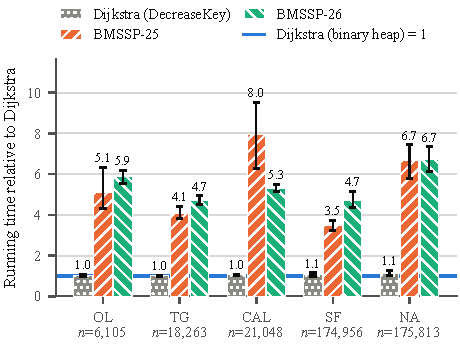
\includegraphics[width=0.62\textwidth]{real_ratio}\end{center}
Each group of bars is one network. The blue line at height 1 is Dijkstra. A bar of height 5 means that algorithm needed five times as long. The thin whiskers show the best and worst source. Reading: \bmA{} is \RealRatioMinTwoFive--\RealRatioMaxTwoFive{} times slower and \bmB{} is \RealRatioMinTwoSix--\RealRatioMaxTwoSix{} times slower than Dijkstra; the two Dijkstra variants are practically equal. \bmB{} beats \bmA{} on only \RealTwoSixFasterWord{} of the five networks.

\subsection{Road networks: counts (paper Table VI and Fig.~1)}
\begin{center}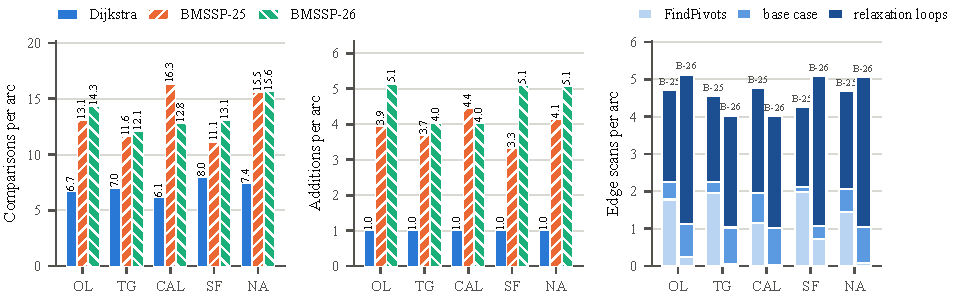
\includegraphics[width=\textwidth]{real_counts}\end{center}
Left and middle panel (in the paper these numbers are Table VI): comparisons and additions per edge. Dijkstra makes 6--8 comparisons and exactly 1 addition per edge. The new algorithms make 11--16 comparisons and 3--5 additions. So on road networks they are slower \emph{already in the abstract cost model}, before any hardware effects.

Right panel (this is Fig.~1 of the paper): how often each edge is scanned, and in which part of the algorithm. Dijkstra: once. \bmA{} (bars marked B-25): 4--5 times, of which more than one whole pass happens inside FindPivots (light blue). \bmB{} (B-26): 4--5 times as well, but almost none of it in FindPivots. This is the clearest picture of what the 2026 paper changed: pivot finding became cheap. The dark part (relaxation loops) is larger for 2026 because every recursion level relaxes every edge once and the 2026 parameters give one more level on three of the five networks.

\emph{Cost per operation.} If an algorithm needs 4.5 times the time but only 2 times the operations, each of its operations costs about 2.3 times as much. This number is \PerOpMinTwoFive--\PerOpMaxTwoFive{} for \bmA{} and \PerOpMinTwoSix--\PerOpMaxTwoSix{} for \bmB. It reflects things the abstract model ignores: bigger labels, bookkeeping, and memory accesses that the processor cannot predict.

\subsection{Validation table (paper Table IV)}
Rows: the algorithm as printed in its paper and with the repairs. Columns: number of runs; runs with a wrong distance (always 0); runs in which a stale key was seen; runs in which a vertex was reported complete twice; runs in which the base-case boundary invariant was violated. Reading: the stale keys occur in both algorithms; without the deletion they cause duplicate completions; with the repairs the duplicate and boundary columns are zero.

On the real road networks these effects are rare (duplicates are at most \DupPctMaxTwoFive\% of the vertices) and make no measurable difference to the running time; they matter for whether the published proofs apply, not for speed.

\subsection{Degree reduction (paper Table VII)}
The proofs assume a graph in which every vertex has very few edges. Transforming the road networks into that form makes them \ReduceNGrowMin--\ReduceNGrowMax{} times larger, and every algorithm becomes several times slower on the transformed graph. Conclusion: the transformation is needed for the proofs, but in practice one should not apply it. (Castro et al.\ found the same for the 2025 algorithm.)

\subsection{Parameter sweep (paper Fig.~2)}
\begin{center}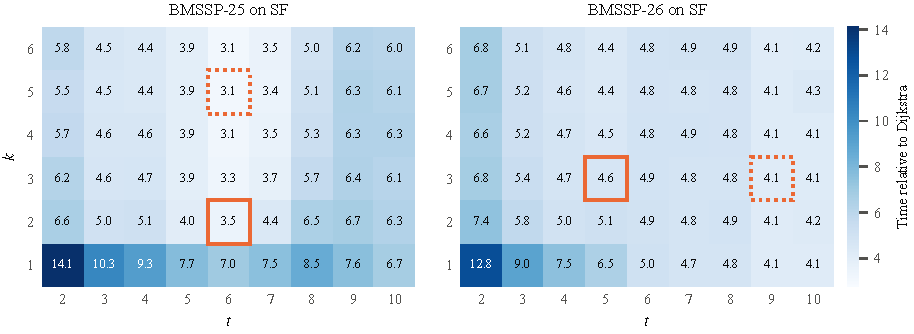
\includegraphics[width=\textwidth]{params_heatmap}\end{center}
Each cell is one choice of $(k,t)$ on the San Francisco network; the number is the time relative to Dijkstra (smaller and lighter is better). The solid orange box is the choice prescribed by the paper, the dotted box the best one found. Reading: $k=1$ (bottom row) is bad, which shows that reducing the frontier really is necessary; the prescribed parameters are reasonable; tuning gains \ParSFTwoFiveGain\% (2025) and \ParSFTwoSixGain\% (2026) on SF and \ParNATwoFiveGain\% and \ParNATwoSixGain\% on NA; but even the best cell is about \ParSFTwoFiveBest{} times slower than Dijkstra.

\subsection{Growing graphs: time (paper Fig.~3)}
\begin{center}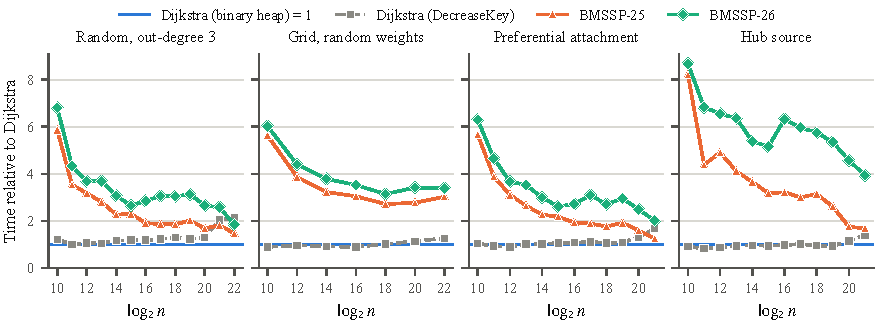
\includegraphics[width=\textwidth]{scaling_ratio}\end{center}
Four families of generated graphs, sizes from about a thousand to about four million vertices (the horizontal axis is $\log_2 n$, so each step doubles the size). Vertical axis: time relative to Dijkstra (blue line at 1). Reading:
\begin{itemize}
\item \emph{Random graphs and preferential-attachment graphs:} the new algorithms catch up steadily as graphs grow. \bmA{} goes from \ScaleRandTwoFiveFirst{} times slower at $2^{10}$ to \ScaleRandTwoFiveLast{} times slower at $2^{22}$ on random graphs, and to \ScaleBaTwoFiveLast{} on the largest preferential-attachment graph. They never get below the blue line.
\item \emph{Grids:} no catching up beyond a certain point; both stay between \GridLateMin{} and \GridLateMax{} times slower.
\item \emph{Hub graphs:} \bmA{} reaches \ScaleHubTwoFiveLast, \bmB{} stays at \ScaleHubTwoSixLast.
\item \bmB{} (green) is above \bmA{} (orange) in every panel: it was slower on all \SynthPoints{} generated graphs.
\item The zig-zags come from rounding: $k$, $t$ and the number of levels are whole numbers and jump at certain sizes.
\end{itemize}

\subsection{Growing graphs: counts (paper Fig.~4)}
\begin{center}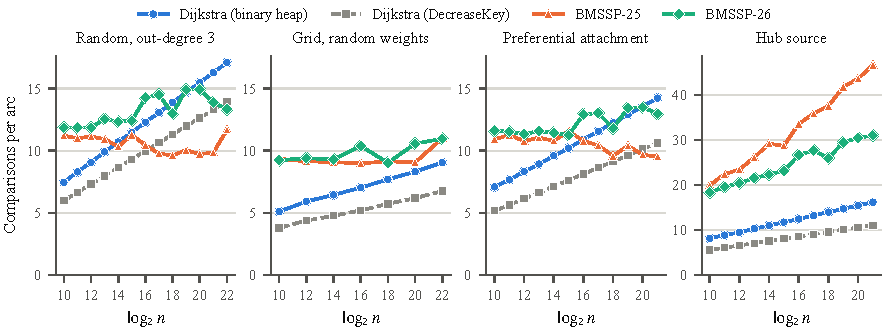
\includegraphics[width=\textwidth]{scaling_cmp}\end{center}
This is the most interesting figure: comparisons per edge as the graphs grow. (The additions per edge are in \code{figure\_data.txt} and are quoted in the text.)
\begin{itemize}
\item On \emph{random} and \emph{preferential-attachment} graphs the blue Dijkstra line climbs steadily (about \SlopeRandDij{} more comparisons per edge every time the graph doubles: that is the $\log n$ of the sorting barrier), while the orange \bmA{} line stays flat at about 10. The lines cross: from $n=2^{\CrossCmpRandTwoFiveDij}$ (random) and $2^{\CrossCmpBaTwoFiveDij}$ (preferential attachment) on, \bmA{} needs fewer comparisons than Dijkstra, and from $2^{\CrossOpsRandTwoFiveDij}$ and $2^{\CrossOpsBaTwoFiveDij}$ on also fewer comparisons plus additions. \bmB{} gets below Dijkstra's comparison count at about a million vertices. \textbf{So the theoretical advantage is real and already visible at ordinary sizes, if one counts operations.}
\item It is still slower on the clock. At $2^{20}$ random vertices \bmA{} performs \OpsRandTwentyTwoFive{} operations per edge against Dijkstra's \OpsRandTwentyDij, yet needs \TimeRandTwentyTwoFive{} times the time. The abstract model does not charge for looking at every edge 3--5 times, for wider labels or for the bookkeeping of the block structures.
\item On \emph{grids} (and road networks) there is no crossing. Reason: Dijkstra's heap stays tiny there (on the largest grid it never holds more than \PeakGrid\% of the vertices; on random graphs \PeakRand\%). With a small heap Dijkstra has almost no sorting work that could be saved.
\item On \emph{hub} graphs (note the different vertical scale) the new algorithms do far more comparisons, although the frontier is as wide as possible. Reason: the source has an edge to every other vertex, which breaks the ``small degree'' assumption. All these edges arrive in the data structure at once and get fully sorted. Paper Table VIII checks this explanation: after the degree-reduction transformation the same graph satisfies the assumption, and then \bmB{} needs less than half of Dijkstra's comparisons (\HubRedCmpTwoSix{} against \HubRedCmpDij{} per original edge). But the transformed graph is eight times larger, so everything is slower than plain Dijkstra on the original graph (\HubCmpDij{} comparisons per edge).
\end{itemize}
\textbf{Take-away on graph structure.} Two properties decide how the new algorithms compare with Dijkstra: how wide Dijkstra's frontier gets (wide is good for the new algorithms), and whether some vertex has a huge degree (bad for them unless the graph is transformed, which is costly).


\subsection{The graphs from bzantium's repository (paper Table IX)}\label{sec:snapex}
Six graphs from the SNAP collection, the same ones bzantium's README uses: two web graphs (Stanford, Google), three road networks (Pennsylvania, Texas, California) and the Pokec social network, with 0.3 to 2 million vertices and up to 30.6 million edges. They have no weights, so each is run twice: with all weights 1 (what bzantium does) and with random weights.

Reading of the table: Dijkstra is the fastest on all \SnapInstances{} instances. \bmA{} is \SnapRatioMinTwoFive--\SnapRatioMaxTwoFive{} times slower and \bmB{} \SnapRatioMinTwoSix--\SnapRatioMaxTwoSix{} times slower. The advantage that bzantium's table shows for its ``V2'' solver therefore does not exist for the real algorithm on the very same graphs.

The comparison counts again follow the frontier rule. The three SNAP road networks have narrow frontiers (at most \SnapRoadPeakMax\% of the vertices) and the new algorithms need more comparisons than Dijkstra (\SnapCmpRoadMinTwoFive--\SnapCmpRoadMaxTwoFive{} times for \bmA). The web and social graphs have wide frontiers (\SnapOtherPeakMin--\SnapOtherPeakMax\%), and there \bmA{} needs between \SnapCmpOtherMinTwoFive{} and \SnapCmpOtherMaxTwoFive{} times Dijkstra's comparisons: fewer than Dijkstra on \SnapFewerCmpTwoFive{} of the \SnapInstances{} instances. So the pattern found on generated graphs also shows on real ones.

\subsection{Density and weight range (paper Section VI-I; this chart is only in the guide)}
\begin{center}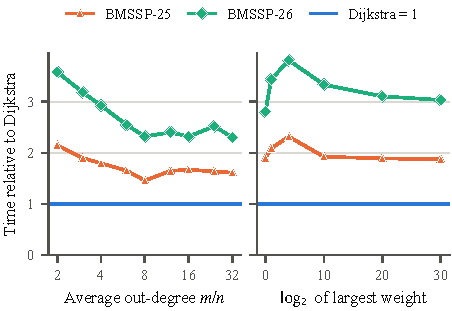
\includegraphics[width=0.62\textwidth]{sweeps}\end{center}
Left: random graphs with more and more edges per vertex. The new algorithms get relatively better up to about 8 edges per vertex and then level off (ratios \DensMinTwoFive--\DensMaxTwoFive{} for 2025, \DensMinTwoSix--\DensMaxTwoSix{} for 2026). Right: the size of the weights hardly matters, not even in the extreme case where all weights are 1 and many comparisons are decided by the tie-breaking rule.

\subsection{Memory (paper Section VI-J)}
On the 4-million-vertex random graph the whole program needed \MemDij~MB with Dijkstra, \MemTwoFive~MB with \bmA{} and \MemTwoSix~MB with \bmB. The extra memory is mainly the per-level lookup tables.


\section{Do other implementations agree, and can ours be trusted?}\label{sec:others}
\subsection{What others found}
\begin{longtable}{@{}p{4.1cm}p{11.1cm}@{}}
\toprule
Source & What it reports, and what I found when reading it\\
\midrule
Castro, Clementino, de Freitas (arXiv:2511.03007; code \code{lcs147/bmssp}, C++) & Faithful implementation of the 2025 algorithm. Dijkstra is 3--4 times faster on large graphs (up to 27.5 times on small grids). \textbf{Agrees with us.}\\
Valko, Paranjpe, Marx G\'omez (arXiv:2509.13448, Rust) & On Lightning Network graphs the 2025 algorithm is consistently slower than Dijkstra. \textbf{Agrees with us.}\\
\code{bzantium/bmssp-python}, solver ``V1'' (educational) & Follows the paper; its README says it is 2--4 times slower than Dijkstra. \textbf{Agrees with us.}\\
\code{bzantium/bmssp-python}, solver ``V2'' (optimized) & README table shows it beating Dijkstra on Stanford, Google, Pokec, LiveJournal. But the code's own documentation calls V2 a ``simplified version'' that ``eliminates the complex multi-level recursion, pivot finding phases'' and the block data structure; it is a bucket queue with fixed bucket width (delta-stepping). The graphs are loaded with \emph{every weight equal to 1}, and one source--target pair is timed. With unit weights a bucket queue is essentially breadth-first search, a linear-time method that only works because the weights are small integers. \textbf{It is not the Duan et al.\ algorithm, so it does not contradict us.}\\
\code{alphastrata/DunMaoSSSP} (Rust) & README: ``15x faster than Dijkstra on LiveJournal''. The benchmark times five random source--target pairs on unit weights against the \code{petgraph} library routine. In the V2 solver, the recursion returns immediately when pivot finding reaches its size limit (the paper continues with all of $S$ as pivots), and its block structure does not keep blocks ordered. The repository's sanity test uses the 3\,353-vertex Rome graph, while V2 answers every graph below 50\,000 vertices with a plain Dijkstra fallback. I did not run it; from the source, it is \textbf{not a faithful implementation}.\\
\code{mfreeman451/bmssp-go} & Claims 1.7--5.5 times speed-up on graphs with at most 2\,500 vertices. Same simplified bucket-queue design as bzantium's V2. \textbf{Not the Duan et al.\ algorithm.}\\
\bottomrule
\end{longtable}
So: every implementation that actually follows the published algorithm finds Dijkstra faster, as we do. The repositories that claim the opposite benchmark a different, simplified algorithm on unit-weight graphs. To be sure, the paper now also runs our implementations on the graphs of bzantium's table (Section~\ref{sec:snapex}): Dijkstra stays faster there too.

\subsection{Is our implementation correct?}
Yes, as far as testing can show: \ValSmallRuns{} + \ValMediumRuns{} validation runs against an independent Bellman--Ford, and every one of the benchmark runs is compared with Dijkstra on all vertices (Section~7). A wrong implementation would give wrong distances somewhere; ours never did.

\subsection{Is it unreasonably slow? (Would a better implementation beat Dijkstra?)}
The best available yardstick is Castro et al.'s implementation, because its structure is the same as ours (I compared the two sources function by function: same parameters $k$, $t$ and levels, same Pull that collects more than $M$ keys from each block sequence, same per-level lookup tables, same deletion fix; the only algorithmic difference is that they track tree roots during the relaxation rounds while we build the forest explicitly as the pseudocode says). Their published times on random graphs with $m=3n$, next to ours:
\begin{center}
\begin{tabular}{@{}lrrrrrr@{}}
\toprule
 & \multicolumn{3}{c}{Castro et al.\ (Intel i5-10400F)} & \multicolumn{3}{c}{ours (Apple M1)}\\
$n$ & Dijkstra & BMSSP & ratio & Dijkstra & BMSSP-25 & ratio\\
\midrule
$2^{16}$ & 10.7 ms & 38.2 ms & 3.6 & \MsSixteenDij{} ms & \MsSixteenTwoFive{} ms & \RatioRandSixteenTwoFive\\
$2^{20}$ & 421 ms & 1286 ms & 3.1 & \MsTwentyDij{} ms & \MsTwentyTwoFive{} ms & \RatioRandTwentyTwoFive\\
$2^{22}$ & 2023 ms & 7703 ms & 3.8 & \MsTwentyTwoDij{} ms & \MsTwentyTwoTwoFive{} ms & \RatioRandTwentyTwoTwoFive\\
\bottomrule
\end{tabular}
\end{center}
Our BMSSP is faster than theirs in absolute time and also relative to Dijkstra, so it is not a weak implementation that makes the new algorithm look bad. (Different machines; I did not execute their code, which would mean running third-party code on your laptop. If you want that cross-check, clone \code{lcs147/bmssp} and run its \code{experiments/experiment.cpp} on a graph written by our generator.)

\subsection{Does it have the time complexity of the papers?}
The honest answer has three parts.
\begin{enumerate}
\item \textbf{The building blocks have the stated costs.} Selection is worst-case linear; the block index is a red-black tree; finding and deleting a key is $O(1)$ through the per-level tables; \textsc{Pull}, \textsc{BatchPrepend} and \textsc{Merge} touch each key a constant number of times plus the tree operations the papers allow; returning a set costs nothing. Nothing in the code does more than the pseudocode asks for, asymptotically.
\item \textbf{Known deviations.} (a) The small local searches use binary heaps where the 2026 paper says Fibonacci heaps; with the tiny heaps involved (at most $k+\delta$ entries) this changes the bound only by a factor that is constant for constant $\delta$. (b) By default the graph is \emph{not} degree-reduced, exactly like Castro et al.'s main variant. The theorems assume bounded degree, so on a graph with a huge-degree vertex the proven bound does not formally apply; the hub experiment (paper Table VIII) shows what then happens, and \code{--reduce} gives the version to which the theorem applies. (c) The three repairs of Section~\ref{sec:fixes}; without the deletion repair the analysis of either paper does not go through.
\item \textbf{The measurements behave like the theory.} A time bound cannot be ``verified'' by experiment, but the counts are consistent with it: on bounded-degree graphs the number of comparisons per edge of both new algorithms stays flat as $n$ grows from $2^{10}$ to $2^{22}$, while Dijkstra's grows by \SlopeRandDij{} per doubling (paper Fig.~4). If our implementation had lost the sub-logarithmic behaviour, its curves would climb like Dijkstra's.
\end{enumerate}

\subsection{Others say ``3--4 times slower''; why does one of our graphs show 8 times?}
Three things explain it, and none of them is a disagreement.
\begin{itemize}
\item \textbf{The ``3--4 times'' is for large graphs.} Castro et al.'s own tables show much larger factors on small ones: 25 times at 128 vertices, 5.8 times at 1\,024 vertices, up to 27.5 times on small grids. Ours start the same way (paper Fig.~3: about 6 at 1\,024 vertices, about 2.3 at 16\,384). Beyond that the two differ: their ratio stays between 2.8 and 3.8 all the way to 33 million vertices, while ours keeps drifting down to 1.5 at 4 million. I cannot tell from their published numbers whether that is the implementation or the machine.
\item \textbf{The 8 is one particular road network (CAL), and it is unusual.} In CAL and NA about \ChainPctA\% and \ChainPctB\% of all vertices have exactly two neighbours: these files store every bend of a road as a vertex, so the graph is mostly long chains. The other three networks have \ChainRestMin--\ChainRestMax\%. On the two chain-like networks \bmA{} is \ChainRatioMin--\ChainRatioMax{} times slower, on the other three \RestRatioMin--\RestRatioMax{} times. Chains are the worst case for the new algorithm relative to Dijkstra: Dijkstra's heap holds almost nothing there, so it is extremely cheap, while the pivot search with $k=2$ only advances two steps along a chain per round. (With a larger $k$ the gap shrinks: on NA the best setting is \ParNATwoFiveGain\% faster than the prescribed one.)
\item \textbf{On ordinary large road networks we get the same as everybody else.} On the three SNAP road networks with 1--2 million vertices \bmA{} is \SnapTimeRoadMinTwoFive--\SnapTimeRoadMaxTwoFive{} times slower than Dijkstra; Castro et al.\ report an average of 3.7 on the U.S.\ road networks.
\end{itemize}
The paper now states this explicitly at the end of Section VI-B.

\subsection{``On large graphs the new algorithms are faster''?}
No. The paper never says that, and it is not what was measured. What the paper says (abstract, Section VI-F, Fig.~4, conclusion) is narrower: on large random-like graphs the 2025 algorithm performs \emph{fewer comparisons} than Dijkstra; it is still \emph{slower on the clock} on every single graph we ran. ``Fewer comparisons'' is the quantity the theorem is about; ``faster'' would be a claim about running time, and for that Dijkstra won everywhere.

\section{Reproducing everything}\label{sec:repro}
Run from the project folder. The scripts needed are exactly the ones listed.
\begin{lstlisting}
sh scripts/fetch_data.sh snap            # 1. download the road networks (+ SNAP graphs)
make -C scripts                          # 2. build bin/sssp and bin/sssp_count
make -C scripts check                    # 3. (optional) sanitizer build + validation
python3 scripts/run_experiments.py       # 4. all measurements -> results/*.csv
python3 -m venv .venv
.venv/bin/pip install matplotlib numpy
sh scripts/build_pdfs.sh                 # 5. figures, tables, numbers.tex and both PDFs
\end{lstlisting}
Step 5 runs \code{scripts/make\_figures.py} (figures, table bodies, \code{paper/numbers.tex}, \code{results/summary.json}) and then typesets \code{paper/main.tex} and \code{explanation/explanation.tex} with Tectonic, writing \code{research-paper.pdf} and \code{explanation.pdf}.
Step 4 takes about an hour on the laptop used here (Apple M1, 8~GB). It skips experiments whose CSV already exists; add \code{--force} to redo them, or name experiments to run only some, for example \code{python3 scripts/run\_experiments.py real params}. The option \code{--counts-only} redoes only the operation counts and leaves the timings untouched. Timings will differ on another machine; the counts in \code{*\_count.csv} and the validation tables will be identical because all random seeds are fixed.

\begin{longtable}{@{}p{2.2cm}p{4.9cm}p{8.1cm}@{}}
\toprule
Experiment & Output files & Used for\\
\midrule
\code{info} & \code{graph\_info.csv} & Table III (road networks)\\
\code{validate} & \code{validation/*.csv}, witness files & Table IV, Section VI-A\\
\code{real} & \code{real\_time.csv}, \code{real\_count.csv} & Tables V and VI, Fig.~1\\
\code{variants} & \code{variants\_*.csv} & last paragraph of Section VI-A\\
\code{reduce} & \code{reduce\_*.csv} & Table VII\\
\code{params} & \code{params\_*.csv} & Fig.~2\\
\code{scaling} & \code{scaling\_*.csv} & Figs.~3 and 4\\
\code{hubreduce} & \code{hubreduce\_*.csv} & Table VIII\\
\code{snap} & \code{snap\_*.csv} & Table IX\\
\code{density}, \code{weights} & \code{density\_*.csv}, \code{weights\_*.csv} & Section VI-I\\
\code{memory} & \code{memory.csv} & Section VI-J\\
\bottomrule
\end{longtable}
No number in the paper's text was typed by hand: \code{make\_figures.py} writes them as LaTeX macros into \code{paper/numbers.tex}, and the text uses the macros.

\section{Redrawing the figures yourself}\label{sec:figdata}
The paper has four figures. Every value plotted in them is in the plain-text file \code{figure\_data.txt} in the project folder, so you can redraw them in Excel, Google Sheets, Origin, gnuplot or anything else without touching the code.
\begin{itemize}
\item The file is tab-separated. Each block starts with a line \code{\#\# FIGURE n: ...} that says what the block is, then a few lines \code{\# HOW TO PLOT} with the chart type, what goes on the x axis and the y axis, which columns are the lines or bars, the scales, and any reference line; then a header line with the column names and the rows. Copying the header and rows into a spreadsheet gives one column per field.
\item \textbf{FIGURE 1} (stacked bars): for each road network and each of the two new algorithms, the edge scans per edge in FindPivots, in the base case and in the relaxation loops. Dijkstra is 1.0 everywhere.
\item \textbf{FIGURE 2} (heat map): one row per algorithm and $k$, one column per $t$; the cell is the time relative to Dijkstra on SF. A second block has the same sweep on NA (quoted in the text).
\item \textbf{FIGURE 3} (line chart, four panels): family, $\log_2 n$, and the time relative to Dijkstra for the three other programs.
\item \textbf{FIGURE 4} (line chart, four panels): family, $\log_2 n$, and comparisons per edge for all four programs (additions per edge are included too).
\item Blocks marked \code{EXTRA} hold the numbers of charts that are \emph{not} figures in the paper (the road-network ratios of Table V with the smallest and largest value over the start vertices, the counts of Table VI, and the density and weight sweeps of Section VI-I), in case you want to draw those as well.
\end{itemize}
The file is rewritten by \code{scripts/make\_figures.py} every time the figures are regenerated, so it always matches the PDF. The complete raw measurements (every single run) are the CSV files in \code{results/}.

Why four figures and not more: a chart was dropped from the paper when a table or a sentence already gave the same numbers (the bar chart of Table V, the bar charts of Table VI, the density and weight curves, and a second row of the comparison chart). Those charts are still shown in this guide.

\section{What was checked against the proposal and the sources}\label{sec:verified}
You asked that nothing be assumed. This is what was verified, and how.
\begin{itemize}
\item \textbf{Both Duan et al.\ papers were read in full} (arXiv 2504.17033v2; arXiv 2602.07868v2 and the published ICALP PDF). The pseudocode used for the implementation is identical in the arXiv and ICALP versions of the 2026 paper.
\item \textbf{Proposal error: the degree parameter.} The proposal prints $\delta=14\min\{m/n,\log\log n\}$. The paper says $\delta=\tfrac14\min\{m/n,\log\log n\}$ (a lost fraction bar). Moreover this value is below the required minimum $3$ for every $n<2^{4096}$, so in practice $\delta=3$; the paper states this.
\item \textbf{Proposal claim ``Dijkstra is three to four times faster in every tested scenario''} (about Castro et al.). That is the wording of their abstract, but their own tables report up to 27.5 times on small grids. The paper quotes both.
\item \textbf{Proposal claim ``road networks up to $10^7$ vertices''.} Castro et al.'s text gives about $2.3\times10^7$ vertices for the largest road network and $2^{25}$ for random graphs; the paper uses the latter figure only.
\item \textbf{Reference [14] of the proposal} has changed its title: arXiv:2509.13448v2 (16 Sep 2026) is called ``An Empirical Evaluation of BMSSP and Dijkstra's Algorithm for the Lightning Network''. The paper cites v2.
\item \textbf{Reference [13] of the proposal} lists five authors including L.~Castro. The package's own citation and Castro et al.'s bibliography list four (Makowski, Guter, Russell, Saragih); SSRN could not be opened to settle this, so the paper cites the four authors and makes no statement about overlapping authorship.
\item \textbf{``No peer-reviewed evaluation of the 2026 algorithm exists.''} This cannot be proved; the paper says ``to our knowledge''.
\item \textbf{Bibliographic data} (authors, venue, pages, DOI) of every journal and conference reference were checked against Crossref or the publisher's page on 12 Oct 2026: STOC~2025 pp.~36--44; ICALP~2026, LIPIcs vol.~374, art.~81, pp.~81:1--81:23; FOCS~2024 pp.~2099--2130; and the classical references.
\item \textbf{The data set.} The repository's files list each road segment once, always with start id $<$ end id. Read as one-way edges the graphs are almost entirely unreachable (6 vertices reachable from vertex 0 in California), read as two-way they are all connected; so every segment is used in both directions. This is stated in the paper.
\item \textbf{The earlier AI runs} in the neighbouring folders were read for orientation only. Their claims about the stale keys and the base case were re-derived from my own instrumented implementation; their numbers are not used anywhere.
\item \textbf{The Dijkstra baseline is not handicapped}: it was timed against \code{std::priority\_queue} and is slightly faster.
\end{itemize}

\section{How the paper refers to the code, and what is left for you}
\textbf{Practice.} Papers do not print file paths. The common forms are a sentence such as ``the code is publicly available at \emph{URL}'' (this is what Castro et al.\ do) or, in IEEE style, a numbered reference to the software. The IEEE Reference Guide has a ``Software'' entry type and follows the FORCE11 Software Citation Principles: name the authors, the software, the repository, a version or date and the address. The paper therefore says once, at the end of the implementation section, that implementations, drivers, raw measurements and figure scripts are publicly available, and cites reference [24]:
\begin{quote}\small
Anmol, Tanmay Arora, Adhyyan, and Pahul Veer Singh Gogna. \emph{bmssp-vs-dijkstra: Implementations, experiments and data \dots} (2026). GitHub. [Online]. Available: \url{https://github.com/anmoltutejagithub/bmssp-vs-dijkstra}
\end{quote}
The road-network data is cited the same way (the SSTD~2005 paper the data owners ask to be cited, plus the GitHub mirror).

\textbf{To do before submitting.}
\begin{enumerate}
\item The repository \code{anmoltutejagithub/bmssp-vs-dijkstra} was created on 12 October 2026 as a \emph{private} repository and contains this folder. Readers of the paper cannot open the link until you make it public (GitHub: Settings $\rightarrow$ General $\rightarrow$ Change repository visibility). Do that before you submit.
\item The author block is a single shared block: the four names on one line, then Department of Computer Science \& Engineering, Chitkara University, Punjab, India, then the four e-mail addresses in the order of the names. The affiliation wording was taken from the example block you showed on 12 October 2026; change it at the top of \code{paper/main.tex} if your department is named differently.
\item Choose a licence for the repository. For long-term citation the usual next step is to archive a release on Zenodo and cite the DOI.
\item Timings come from one laptop. If a reviewer asks, re-run step 4 on a second machine; the counts will not change.
\end{enumerate}

\section{Limits of what the study shows}
\begin{itemize}
\item One machine, one compiler; absolute times are specific to it. The operation counts are not.
\item The implementations follow the pseudocode and are reasonably engineered, but they are not tuned to the limit. The counts show that a large part of the gap cannot be engineered away because it is extra work prescribed by the algorithms.
\item Weights are integers (an exact subset of the real numbers); floating-point rounding was not studied.
\item The largest graphs have $2^{22}$ vertices because of the 8~GB of memory. Nothing is claimed about where, if anywhere, a crossover would occur.
\item The two observations on the 2026 pseudocode are empirical findings on an independent implementation, not statements confirmed by its authors.
\end{itemize}

\section{Glossary}
\begin{description}[style=nextline,leftmargin=1.2cm]
\item[arc] a directed edge.
\item[{label $\dhat[v]$}] best known path length to $v$; never below the true distance $d(v)$.
\item[relaxation] trying to improve $\dhat[v]$ through an edge $(u,v)$.
\item[complete] a vertex whose label equals its true distance.
\item[frontier] vertices through which all unfinished shortest paths must pass.
\item[BMSSP] bounded multi-source shortest path: the recursive sub-problem of both new algorithms.
\item[pivot] a frontier vertex kept for the recursion after the frontier has been thinned out.
\item[$k$, $t$] the two parameters: $k$ controls how hard pivot finding works, $2^t$ is the fan-out of the recursion.
\item[$\delta$] the degree bound assumed by the 2026 analysis.
\item[partial execution] a call that stops early and returns a bound $B'<B$.
\item[stale key] an entry of the structure $D$ whose stored value is larger than the current label of its vertex.
\item[edge scan] one look at an edge in any loop of an algorithm (Dijkstra: exactly one per edge).
\item[comparison-addition model] the cost model of the theorems: only additions and comparisons of weights are counted.
\end{description}

\end{document}
